%%% Esqueleto base de la presentacion
%%% No agregar las paginas con un include
%%% Lo que quieran aportar deben ser usuarios del TRAC

\documentclass{beamer}
\usepackage[spanish,activeacute]{babel}
\usepackage[utf8]{inputenc}
\usepackage{listings}
\usepackage{color}
\definecolor{gray2}{rgb}{100,100,100}
\definecolor{red}{rgb}{255,0,0}
\definecolor{green}{rgb}{0,1,0} 
\definecolor{blue}{rgb}{0,0,1} 
\newcommand{\blue}{\textcolor{blue}}
\newcommand{\red}{\textcolor{red}}
\newcommand{\green}{\textcolor{green}}



\usetheme[pageofpages=of,% String used between the current page and the
                         % total page count.
          alternativetitlepage=true,% Use the fancy title page.
          titlepagelogo=img/bio,% Logo for the first page.
          watermark=img/bio-off,% Watermark used in every page.
          watermarkheight=100pt,% Height of the watermark.
          watermarkheightmult=4,% The watermark image is 4 times bigger
                                % than watermarkheight.
          ]{Torino}

\usecolortheme{nouvelle}
\vspace{-0.5cm}
\author{\large Rodrigo Fernández\\ Cristián Maureira\\Gabriel Zamora}
\title{\Huge Genoma y Ensamblado}
\subtitle{Seminario de Modelos y Métodos cuantitativos (Bioinformática)}
\institute{Universidad Técnica\\Federico Santa María}

\begin{document}
%%%%%%%%%%%%%%%%%%%%%%%%%%
%Definicion de la portada%
%%%%%%%%%%%%%%%%%%%%%%%%%%
\begin{titlepage}
    \begin{center}
	%\begin{tabular}{ccc}
	\begin{tabular}{c}
		
\includegraphics[width=0.9\textwidth]{img/logos}
		
	   % 
\includegraphics[width=3cm]{img/utfsm}
	   % & 
	   % \hspace{-0.2cm}
	   % \begin{tabular}{c}
	   % Universidad Técnica Federico Santa María \\ \hline
	   % \vspace{0.2cm}
	   % Departamento de Informática\\
	   % \vspace{1.2cm}
	   % \end{tabular}
	   % \hspace{0.2cm}
	   % &
        %    
\includegraphics[width=2cm]{img/di}
	\end{tabular}

	\vspace{4cm}
	%Titulo del Documento
	\begin{tabular}{c}
		\vspace{3cm}
		\Large{\sc{Seminario de Modelos y Métodos Cuantitativos}}\\
		\huge{\sc{Tarea 2}}\\\\
		%\includegraphics[scale=0.7]{img/portada} \\\\
	\end{tabular}

    \vspace{5cm}
	\begin{tabular}{lr}
			\textbf{Alumnos} & \\
							 & \\
         	\normalsize{Cristián Maureira Fredes} & \url{cmaureir@csrg.inf.utfsm.cl}\\
         	\normalsize{Gabriel Zamora Nelson} & \url{gzamora@csrg.inf.utfsm.cl}\\

							 & \\
			\textbf{Profesor} & \\
							 & \\
         	\normalsize{Andrés Moreira} & \url{amoreira@inf.utfsm.cl}\\
	\end{tabular}

\vspace{2cm}

	%Fecha
    \normalsize{\sc{\today}}\\
    %\normalsize \textbf{Fecha de Entrega:} & {14 de Noviembre del 2010}\\
    \end{center}
\end{titlepage}

\tableofcontents

%\begin{frame}
%\frametitle{...}
%\framesubtitle{...}
%
%\end{frame}

\section{Genoma}
% buscar en el genbank de mbi

\begin{frame}
\begin{center}
	\Huge{Genoma}
\end{center}
\end{frame}


\begin{frame}
\frametitle{Genoma}
\framesubtitle{¿Qué es?}
\begin{itemize}
    \item \textbf{Totalidad} de la información genética que posee un organismo en
		particular.
    \begin{itemize}
        \item No olviden al genoma Mitocondrial!
    \end{itemize}
\end{itemize}
\begin{center}
	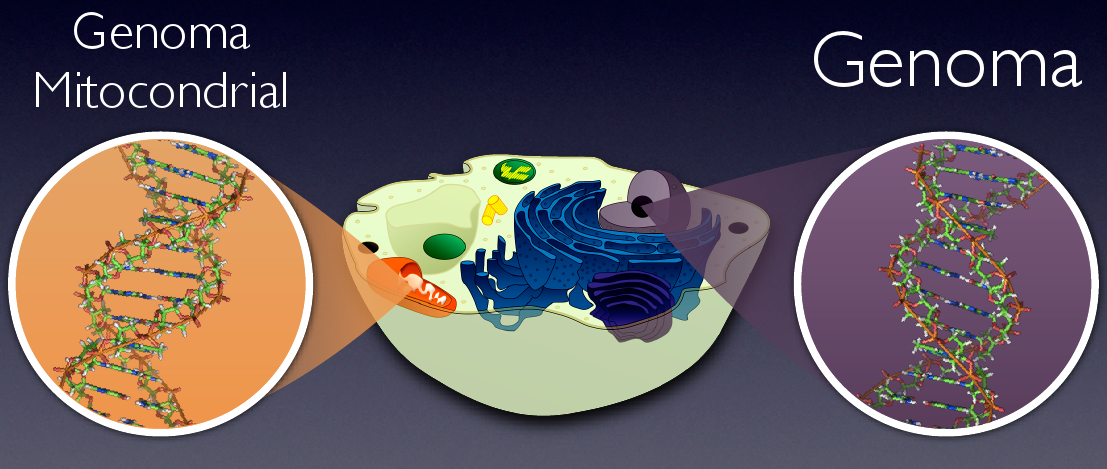
\includegraphics[width=0.9\textwidth]{img/genomas}
\end{center}
\end{frame}


\begin{frame}
\frametitle{Genoma}
\framesubtitle{¿Qué contiene?}
\begin{columns}
\begin{column}{0.7\textwidth}
	\begin{itemize}
	    \item \textbf{Genes} que codifican \textbf{proteínas}.
	    \item ``Genes'' que codifican \textbf{RNA's estructurales}: rRNA, tRNA, etc.
	    \item Secuencias de \textbf{control}.
	    \item En general, mucha \textbf{basura}.
	    \begin{itemize}
	        \item Repeticiones de secuencias.
	        \item Hartas A y T (en relación a la estructura de la cromatina).
	        \item Duplicados en desuso.
	        \item Minisatélites, Microsatélites.
	        \item Largo etc.
	    \end{itemize}
	\end{itemize}
\end{column}
\begin{column}{0.3\textwidth}
	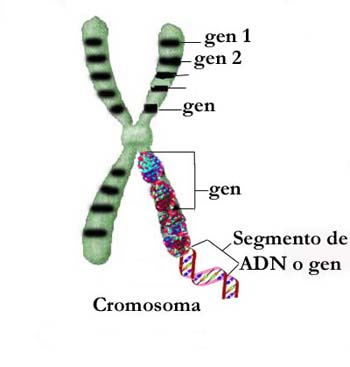
\includegraphics[width=0.95\textwidth]{img/gen.jpg}
\end{column}
\end{columns}
\end{frame}

\begin{frame}
\frametitle{Genoma}
\framesubtitle{¿Qué contiene?}
\begin{center}
	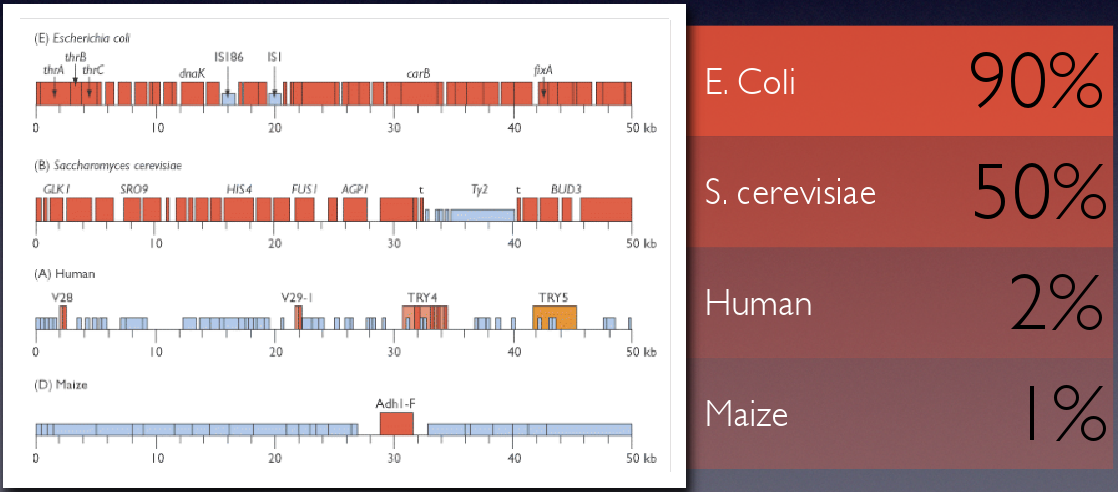
\includegraphics[width=0.95\textwidth]{img/genes}
\end{center}
\end{frame}

\begin{frame}
\frametitle{Genoma}
\framesubtitle{¿Para que sirve?}
\begin{columns}
\begin{column}{0.7\textwidth}
\begin{itemize}
    \item \textbf{Diagnóstico} y \textbf{prevención} de enfermedades\\
%    \begin{itemize}
%        \item Prueba genética
%%las pruebas basadas en el ADN son casi el primer uso
%%comercial y de aplicación médica de los nuevos descubrimientos en genética.
%%Estos ensayos se pueden usar para el diagnóstico de enfermedades, la
%%confirmación diagnostica, la información del pronóstico así como del curso de
%%la enfermedad, para confirmar la presencia de enfermedad en pacientes
%%asintomáticos y, con variados grados de certeza, para predecir el riesgo de
%%enfermedades futuras en personas sanas y en su descendencia.
%    \end{itemize}
    \item Estudio de \textbf{susceptibilidad} en las enfermedades
    \item Intervención (\textbf{tratamiento}) sobre la enfermedad.
    \begin{itemize}
        \item Enfermedades hereditarias.
        \item La ``terapia génica''.
        \item Fármacos a la medida.
    \end{itemize}
\end{itemize}
\end{column}
\begin{column}{0.3\textwidth}
	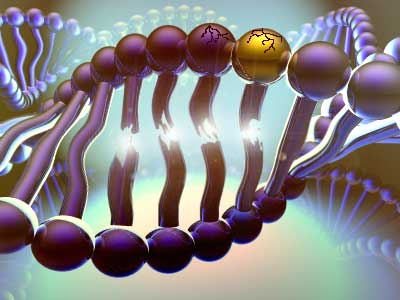
\includegraphics[width=0.95\textwidth]{img/autismo.jpg}
\end{column}
\end{columns}
\end{frame}

\begin{frame}
\frametitle{Genoma}
\framesubtitle{Otros Beneficios...}
\begin{columns}
\begin{column}{0.6\textwidth}
\begin{itemize}
    \item Medicina molecular.
    \item Genómica microbiana.
    \item Valoraciones de riesgo.
    \item Bioarqueología, antropología, \textbf{evolución}...
    \item \textbf{Identificación} ADN.
    \item \textbf{Agricultura} y \blue{bioprocesamiento}.
\end{itemize}
\end{column}
\begin{column}{0.4\textwidth}
	\begin{center}
		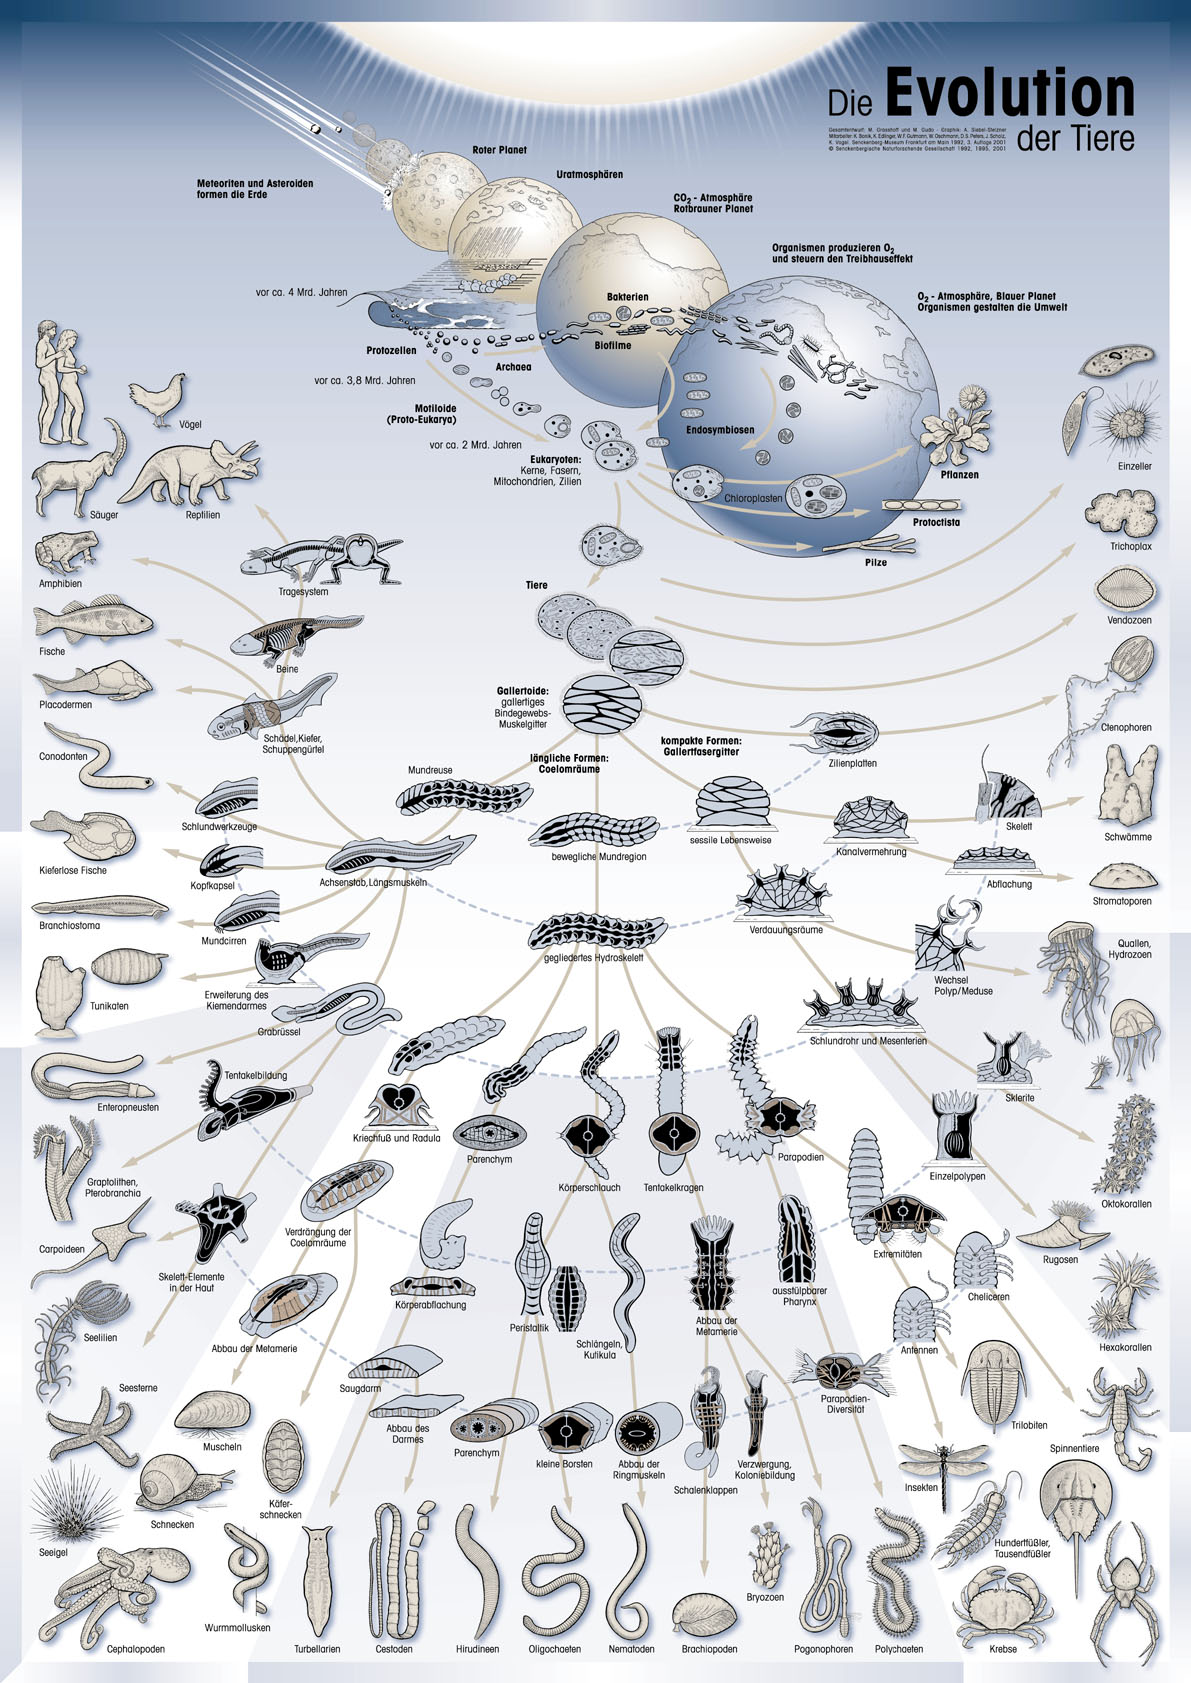
\includegraphics[width=0.95\textwidth]{img/evolution.jpg}
	\end{center}
\end{column}
\end{columns}
\end{frame}

\begin{frame}
\frametitle{Genoma}
\framesubtitle{Eucariotas}

\begin{columns}
\begin{column}{0.5\textwidth}
	\begin{itemize}
	    \item Uno o más \textbf{cromosomas} de DNA lineal.
	    \item De cada cromosoma, un par en cada célula.
	    \item Todos contenidos en el \textbf{núcleo}.
	    \item Los \textbf{genes} (codificando proteínas) ocupan un porcentaje pequeño del
	        DNA.
	    \item Los genes suelen estar interrumpidos por \textbf{intrones}.
	    \item \textbf{Mayor tamaño} que en los procariotas.
	\end{itemize}
\end{column}
\begin{column}{0.5\textwidth}
	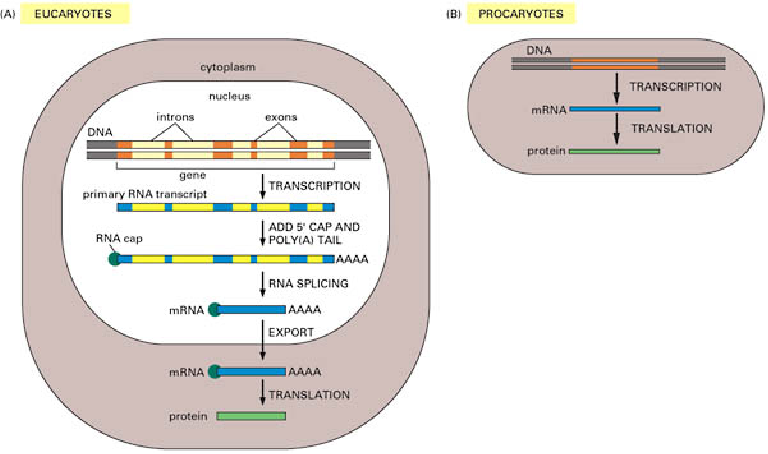
\includegraphics[width=0.95\textwidth]{img/eucariota_procariota}
\end{column}
\end{columns}
\end{frame}

\begin{frame}
\frametitle{Genoma}
\framesubtitle{Procariotas}
\begin{columns}
\begin{column}{0.5\textwidth}
\begin{itemize}
    \item Doble hélice Circular.
    \item \textbf{Flota} ``por ahí''.
    \item Suelen haber \textbf{plásmidos}.
\end{itemize}
\end{column}
\begin{column}{0.5\textwidth}
	\begin{center}
		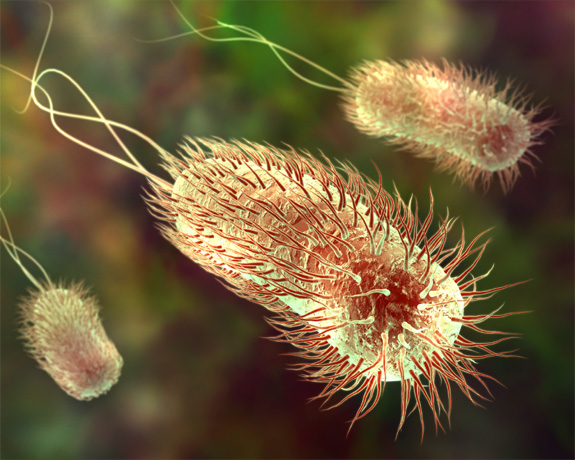
\includegraphics[width=0.95\textwidth]{img/procariota.jpg}
	\end{center}
\end{column}
\end{columns}
\end{frame}

\begin{frame}
\frametitle{Genoma Humano}
\framesubtitle{Algunos datos}
\begin{columns}
\begin{column}{0.7\textwidth}
	\begin{itemize}
	    \item \textbf{38.000} genes (app. \textbf{2\%} de todo el genoma).
	    \item 98\% idéntico al de los \textbf{chimpancés} y otros primates. 99,99\% de
	    similitud entre seres humanos. 
	    \item Se han encontrado 223 genes humanos que resultan similares a los
	    genes \textbf{bacterianos}. (hasta ahora)
	    \item \textbf{5 \%} del genoma codifica \textbf{proteínas}.
	\end{itemize}
\end{column}
\begin{column}{0.3\textwidth}
\begin{center}
	
\includegraphics[width=0.95\textwidth]{img/genoma_humano.jpg}\\
\end{center}
\end{column}
\end{columns}
\end{frame}

\begin{frame}
\frametitle{Genoma Humano}
\framesubtitle{Algunos datos}
\begin{columns}
\begin{column}{0.7\textwidth}
	\begin{itemize}
	    \item  El \textbf{25\%} del genoma humano está casi \textbf{desierto}, existiendo largos espacios libres entre un gen y otro.
	    \item \textbf{35\%} + del genoma contiene secuencias \textbf{repetidas} (ADN basura)
	    \item \textbf{250-300.000} proteínas distintas.
	    \begin{itemize}
	        \item Por tanto cada gen podría estar
	        implicado por término medio en la síntesis de unas \textbf{diez} proteínas.
	    \end{itemize}
	    \item Entre \textbf{1,4 a 2,1} millones de variaciones de un sólo
        nucleótido en el genoma. (hasta ahora)
	\end{itemize}
\end{column}
\begin{column}{0.3\textwidth}
	\begin{center}
		
\includegraphics[width=0.95\textwidth]{img/genoma-humano.jpg}
	\end{center}
\end{column}
\end{columns}
\end{frame}


\begin{frame}
\frametitle{Genoma}
\framesubtitle{Información General}
\begin{columns}
\begin{column}{0.7\textwidth}
	\begin{itemize}
	    \item El récord en tamaño de genoma lo tiene la \textbf{ameba}, con
	    \textbf{670 Gbp} (versus 3 Gbp del
	humano).
	    \item El récord de \textbf{cantidad de genes} va para un cierto
	    \textbf{protozoo}, con \textbf{60.000} (el
		triple que nosotros).
	\end{itemize}
\end{column}
\begin{column}{0.3\textwidth}
\begin{center}
	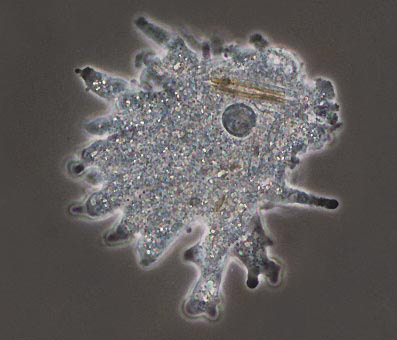
\includegraphics[width=0.95\textwidth]{img/ameba.jpg}
\end{center}
\end{column}
\end{columns}
\end{frame}

\begin{frame}
\frametitle{Genoma}
\framesubtitle{Información General}
\begin{center}
	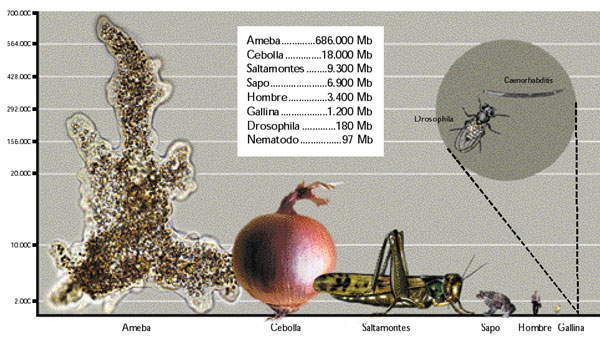
\includegraphics[width=0.95\textwidth]{img/tamanos.jpg}
\end{center}
\end{frame}

\begin{frame}
\frametitle{Genoma}
\framesubtitle{Información General 2}
\begin{columns}
\begin{column}{0.7\textwidth}
	\begin{itemize}
	    \item Las \textbf{vacas} tienen \textbf{60} cromosomas; el \textbf{pez
	    dorado}, alrededor de \textbf{100}.
	    \item Lo único que sí es cierto es que en \textbf{procariotas} el tamaño
	    oscila \textbf{entre 1 y 100} Mbp.
	    \item Y que las cosas que \textbf{vuelan} suelen tener genomas
	    relativamente \textbf{pequeños}.
	\end{itemize}
\end{column}
\begin{column}{0.3\textwidth}
\begin{center}
	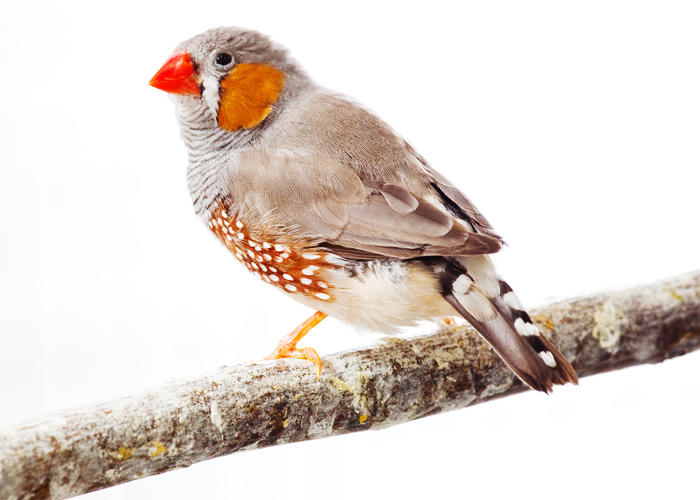
\includegraphics[width=0.95\textwidth]{img/ave.jpg}\\
\end{center}
\end{column}
\end{columns}
\end{frame}

\begin{frame}
\frametitle{Genoma}
\framesubtitle{Información General 3}
\begin{center}
	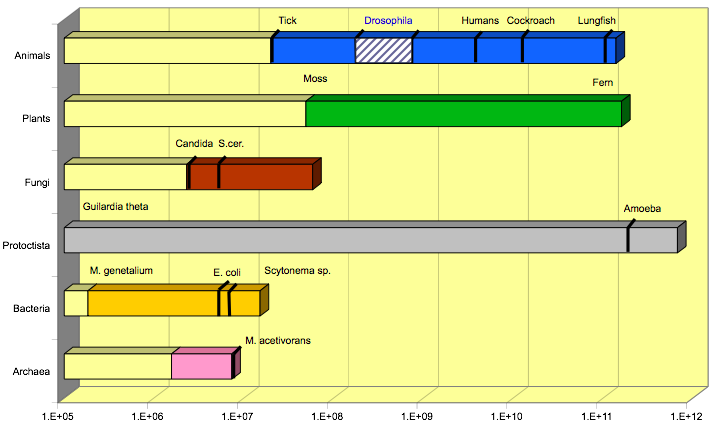
\includegraphics[width=0.95\textwidth]{img/gen_clados}
\end{center}
\end{frame}

\section{Secuenciación}
% que es
\frame
{
\frametitle{Secuenciación de ADN}
\begin{center}
	\huge{¿Qué es?}
\end{center}
}

\frame
{
\frametitle{Secuenciación de ADN}
\framesubtitle{¿Qué es?}
\begin{center}
	\huge{Video}
\end{center}
}


\frame
{
\frametitle{Secuenciación de ADN}
\framesubtitle{¿Qué es?}
\begin{itemize}
	\item Conjunto de métodos y técnicas bioquímicas,
		cuya \red{finalidad} es la \blue{determinación del orden} de los nucleótidos (A, C, G y T) en un oligonucleótido de ADN.
	\item La secuencia de ADN constituye la \blue{información genética heredable} (en núcleo celular, plásmidos, mitocondria,
		y cloroplastos) \red{base de desarrollo} de los seres vivos.
\end{itemize}
}

% para que sirve

\frame
{
\frametitle{Secuenciación de ADN}
\begin{center}
	\huge{¿Para qué sirve?}
\end{center}
}
\frame
{
\frametitle{Secuenciación de ADN}
\framesubtitle{¿Para qué sirve?}
\begin{itemize}
	\item Comprensión.
	\item \red{Atajo!} ayuda a los científicos a encontrar a los genes más fácil y rápidamente.
	\item Hay \blue{pistas} para encontrar los genes.
	\item Se espera que sirva para comprender el \red{todo}.\\

	\begin{center}
	\emph{``...cómo los genes trabajan juntos para dirigir el crecimiento,
		desarrollo y mantenimiento de un organismo entero.''}
	\end{center}
\end{itemize}
}

\frame
{
\frametitle{Secuenciación de ADN}
\framesubtitle{¿Para qué sirve?}
\begin{itemize}
	\item Los genes son el $5\%$ del ADN, la secuencia \red{ayudará} a estudiar
		la parte del genoma por afuera de los genes.
	\begin{itemize}
		\item Sitios \blue{reguladores} que controlan la activación/desactivación de genes.
		\item ADN \blue{sin} sentido.
	\end{itemize}
\end{itemize}
}

% como se hace

\frame
{
\frametitle{Secuenciación de ADN}
\begin{center}
	\huge{¿Cómo se hace?}
\end{center}
}
\frame
{
\frametitle{Secuenciación de ADN}
\framesubtitle{¿Cómo se hace?}
\begin{itemize}
	\item Se secuencia en \emph{partes}.
	\item \red{No} se puede completo (\blue{limitación} métodos sólo con fragmentos)
	\item Fragmentar en pedazos \emph{pequeños}, secuenciarlos y reconstruirlos en orden.
	\item Dos técnicas más utilizadas \emph{(con ventajas y desventajas)}.
	\begin{itemize}
		\item Shotgun.
		\item Hierarchical Shotgun.
	\end{itemize}
	\item La secuenciación del genoma humano ha involucrado una combinación de \blue{ambas} técnicas. 
\end{itemize}
}

% como funciona
\frame
{
\frametitle{Secuenciación de ADN}
\begin{center}
	\huge{¿Cómo funciona?}
\end{center}
}
\frame
{
\frametitle{Secuenciación de ADN}
\framesubtitle{¿Cómo funciona?}
\begin{enumerate}
	\item<1-> Electroforesis para \blue{separar} los fragmentos de ADN.% que difieren en longitud por una base.
	\begin{itemize}
		\item \emph{Técnica para la separación de moléculas según movilidad en un campo eléctrico}.
	\end{itemize}
	\item<2-> Por lo que el ADN a secuenciar se coloca en un \blue{extremo} del gel.
	\item<3-> Electrodos en los extremos (aplicamos \blue{corriente}).
	\item<4-> Migración de fragmentos de ADN por \blue{tamaño} (a través del gel).
\end{enumerate}
}

\frame
{
\frametitle{Secuenciación de ADN}
\framesubtitle{¿Cómo funciona?}
\begin{itemize}
	\item Electroforesis es capaz \red{sólo} de separar fragmentos de 500 pares de bases (justificación anterior!).
	\item \red{Dato:} Hasta 1980, las electroforesis eran leídas por una \blue{persona}.
	\item Hoy en día el proceso es \emph{automático}.
	\item En producir una secuencia de 20.000 a 50.000 bases (Persona $\rightarrow$ 1 año, Máquina $\rightarrow$ horas).
	\item Máquinas con diseño \blue{basado} en el proceso manual.
\end{itemize}
}

\frame
{
\frametitle{Secuenciación de ADN}
\framesubtitle{¿Cómo funciona?}
\begin{itemize}
	\item Usando máquinas. 
	\begin{enumerate}
		\item<1-> Se ubica el gel en un espacio entre dos vidrios de medio milímetro.
		\item<2-> Se espera que el gel se endurezca
		\item<3-> El ADN se siembra en cada una de las 96 calles que corren a lo largo del gel.
		\item<4-> Se aplica corriente eléctrica.
		\item<5-> Los fragmentos de ADN migran de acuerdo a su tamaño.
		\item<6-> La máquina lee el orden de las bases de ADN y guarda la información. 
	\end{enumerate}
\end{itemize}
}

% como se reconoce una base

\frame
{
\frametitle{Secuenciación de ADN}
\begin{center}
	\huge{¿Cómo se reconoce una base?}
\end{center}
}

\frame
{
\frametitle{Secuenciación de ADN}
\framesubtitle{¿Cómo se reconoce una base?}
\begin{itemize}
	\item Secuenciadores automáticos \red{no} ven al ADN (hay que \blue{prepararlo})
	\item El ADN debe estar
	\begin{itemize}
		\item fragmentado
		\item copiado
		\item modificado químicamente
		\item unido a fragmentos fluorescentes (por bases)
	\end{itemize}
	\item Luego del procedimiento, se reconocen por la \blue{fluorescencia} (láser).
\end{itemize}
}

%\frame
%{
%\frametitle{Secuenciación de ADN}
%\framesubtitle{¿Cómo se reconoce una base?}
%\begin{itemize}
%	\item Antes de ser secuenciado, un fragmento de ADN se copia muchas veces,
%		luego se divide en cuatro partes para otra fase de copiado.
%	\item En esta segunda fase de copiado, se agrega una pequeña cantidad de base
%		químicamente modificada a cada parte (o sea, A modificada a una parte,
%		C modificada a otra y así sucesivamente).
%	\item Cuando una de estas bases modificadas es incorporada en la molécula de ADN,
%		la cadena de bases se frena.
%\end{itemize}
%}
%
%\frame
%{
%\frametitle{Secuenciación de ADN}
%\framesubtitle{¿Cómo se reconoce una base?}
%\begin{itemize}
%	\item El resultado de todo esto es que una parte contendrá solo fragmentos que
%		terminen en A, otra parte fragmentos que terminen en C y así sucesivamente.
%	\item Además, en la segunda fase de copiado, se le agrega un tinte fluorescente
%		distinto a cada parte. 
%	\item Luego se siembra en una misma calle una mezcla de las cuatro partes.
%\end{itemize}
%}
%
%\frame
%{
%\frametitle{Secuenciación de ADN}
%\framesubtitle{¿Cómo se reconoce una base?}
%\begin{itemize}
%	\item Como las moléculas más pequeñas migran más rápido,
%		los fragmentos de ADN se leen en orden creciente de tamaño,
%		cada fragmento con una base más que el anterior.
%	\item A medida que los fragmentos migran, un láser detecta los tintes de las
%		moléculas fluorescentes y así se corresponde con la base: A, C, T o G. 
%\end{itemize}
%}

% que ocurre despues

\frame
{
\frametitle{Secuenciación de ADN}
\begin{center}
	\huge{¿Qué ocurre después?}
\end{center}
}

\frame
{
\frametitle{Secuenciación de ADN}
\framesubtitle{¿Qué ocurre después?}
\begin{itemize}
	\item Salida del secuenciador automático.
	\begin{itemize}
		\item Llegan a una \blue{secuencia cruda} (agujeros, errores y ambigüedades).
		\item Proceso de \blue{limpieza} y \blue{ordenamiento} (cuidado con el tiempo)
	\end{itemize}
\end{itemize}
}

\frame
{
\frametitle{Secuenciación de ADN}
\framesubtitle{¿Qué ocurre después?}
\begin{itemize}
	\item Ordenamiento.
	\begin{itemize}
		\item Mediante un programa.
		\item El programa busca y analiza \blue{superposiciones} o secuencias \blue{idénticas} de ADN en diferentes fragmentos.
		\item Los fragmentos que contienen superposiciones se encuentran \red{juntos} en la secuencia final.
	\end{itemize}
\end{itemize}
}

\frame
{
\frametitle{Secuenciación de ADN}
\framesubtitle{¿Qué ocurre después?}
\begin{itemize}
	\item Aceptar o rechazar.
	\begin{itemize}
		\item Genoma no secuenciado \red{no} garantiza ser correcto.
		\item Pueden ocurrir \red{errores} (fragmenta el ADN, copia, secuencia u ordena).
		\item \blue{Truco:} secuenciar el genoma más de una vez. 
		\item Luego del ordenamiento, sigue el proceso de terminación. (no tenemos intuición)
	\end{itemize}
\end{itemize}
}

% distincion

\frame
{
\frametitle{Secuenciación de ADN}
\begin{center}
	\huge{¿Qué hace la secuenciación del genoma humano distinto?}
\end{center}
}

\frame
{
\frametitle{Secuenciación de ADN}
\framesubtitle{¿Qué hace la secuenciación del genoma humana distinto?}
\begin{itemize}
	\item El genoma humano es mucho más \blue{grande} que los genomas que se habían secuenciado anteriormente.
	\item Los anteriores secuenciados eran virus, bacterias u otros organismos simples.
	\item Genoma humano posee 25\% a 50\% de ADN repetitivo, bacterias y virus no mucho.
	\item El ADN repetitivo no sólo es difícil de ordenar sino también de secuenciar.
\end{itemize}
}

\section{Shotgun Sequencing}
%El método desarrollado y preferido por Celera se llama 
%simplemente secuenciación shotgun. Este enfoque fue desarrollado 
%y perfeccionado en los genomas procariotas que son más pequeños en
% tamaño y contienen ADN menos repetitivas. secuenciación aleatoria
% escopeta cizalla ADN genómico en trozos pequeños que están clonados
% en plásmidos y secuenciado en ambas cadenas, lo que elimina el paso
% de BAC del planteamiento del PGH es. Una vez que las secuencias se 
%obtienen, son alineados y montados en la secuencia final.

\frame
{
\begin{center}
	\Huge{Técnicas}\\
	\huge{Shotgun Sequencing}
\end{center}
}

\frame
{
\frametitle{Shotgun Sequencing}
\framesubtitle{¿Qué es?}

\begin{itemize}
	\item Método de secuenciado de ADN, desarrollado y preferido por ``Celera Genomics'', una empresa estadounidense.
	\item Conocido también como ``shotgun cloning''
\end{itemize}

}

\frame
{
\frametitle{Shotgun Sequencing}
\framesubtitle{Ventajas y Desventajas}

\begin{itemize}
	\item Ventajas:
		\begin{itemize}
			\item Moderadamente rápido en procesamiento
		\end{itemize}
	\item Desventajas:
		\begin{itemize}
			\item Problemas con secuencias con repetición.
			\item No detecta secuencias repetidas. Para aquello se basa en datos públicos.
		\end{itemize}
\end{itemize}

}

\frame
{
\frametitle{Shotgun Sequencing}
\framesubtitle{Descripción}
\begin{center}
	\huge{Video}	
\end{center}

}

\frame
{
\frametitle{Shotgun Sequencing}
\framesubtitle{Descripción}

Tomando como ejemplo un genoma trozado en 9 partes:\\

\begin{center}
	
\includegraphics[width=0.5\textwidth]{img/tecnica1-1.png}
\end{center}
}

\frame
{
\frametitle{Shotgun Sequencing}
\framesubtitle{Descripción}

\begin{center}
	\huge ¿Cuantas posibles combinaciones podemos formar?
\end{center}
}

\frame
{
\frametitle{Shotgun Sequencing}
\framesubtitle{Descripción}

\begin{center}
	\huge $9 * 8 * 7 * ... * 2 * 1 = 9! = 362880$
\end{center}
}

\frame
{
\frametitle{Shotgun Sequencing}
\framesubtitle{Descripción}

Dejando de lado la cantidad.\\

\begin{center}
	\huge ¿Como saber cual es la combinación correcta?
\end{center}
}

\frame
{
\frametitle{Shotgun Sequencing}
\framesubtitle{Descripción}

\begin{center}
	
\includegraphics[width=0.5\textwidth]{img/tecnica1-2.png}
\end{center}

}

\frame
{
\frametitle{Shotgun Sequencing}
\framesubtitle{Descripción}

\begin{center}
	
\includegraphics[width=0.5\textwidth]{img/tecnica1-3.png}
\end{center}

}

\frame
{
\frametitle{Shotgun Sequencing}
\framesubtitle{Descripción}

\begin{center}
	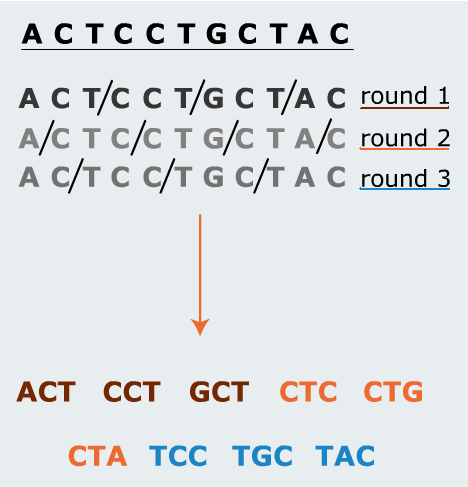
\includegraphics[width=0.5\textwidth]{img/tecnica1-4.png}
\end{center}

}

\frame
{
\frametitle{Shotgun Sequencing}
\framesubtitle{Descripción}

Luego se crea un grafo dirigido:

\begin{itemize}
	\item Sea $x_i = c_{i1} c_{i2} ... c_{in-1} c_{in}$ el contenido de un estado $i$ en el grafo
	\item Para ir de un estado $i$ a un estado $j$, es necesario que: $x_{in-1}x_{in} = x_{j1} x_{j2}$
	\item Finalmente se busca un ciclo hamiltoneano en dicho grafo, correspondiente a la secuencia buscada.
\end{itemize}
}


\frame
{
\frametitle{Shotgun Sequencing}
\framesubtitle{Descripción}

\begin{center}
	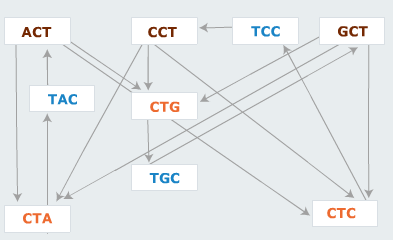
\includegraphics[width=0.7\textwidth]{img/tecnica1-5.png}
\end{center}

}

\frame
{
\frametitle{Shotgun Sequencing}
\framesubtitle{Descripción}

\begin{center}
	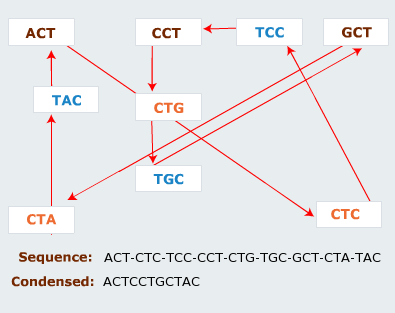
\includegraphics[width=0.7\textwidth]{img/tecnica1-6.png}
\end{center}
}

\section{Hierarchical Shotgun Sequencing}
\frame
{
\begin{center}
	\Huge{Técnicas}\\
	\huge{Hierarchical Shotgun Sequencing}
\end{center}
}

\frame
{
\frametitle{Hierarchical Shotgun Sequencing}
\framesubtitle{¿Qué es?}
\begin{itemize}
	\item También conocida como técnica del \emph{``clon-por-clon''}
	\item Es el método \red{preferido} por el Proyecto del Genoma Humano.
	\item Por lo general es utilizado en genomas con \blue{repeticiones}.
	\item Es \blue{recomendable} utilizar en Eucariontes en general.
	\item Utiliza enzimas en su proceso.
\end{itemize}
}


\frame
{
\frametitle{Hierarchical Shotgun Sequencing}
\framesubtitle{Ventajas y Desventajas}
\begin{itemize}
	\item \blue{Ventajas:}
	\begin{itemize}
		\item Detecta secuencias repetidas.
		\item No tiene problemas de regiones poco representadas.
	\end{itemize}
	\item \red{Desventajas:}
	\begin{itemize}
		\item Demora mucho tiempo.
		\item Posee mucho costo computacional.
	\end{itemize}
\end{itemize}
}


\frame
{
\frametitle{Hierarchical Shotgun Sequencing}
\framesubtitle{¿Cómo funciona?}
\begin{enumerate}
	\item<1-> Construir una \blue{genoteca} por fragmentación del ADN (utilizando BACs)
	\begin{itemize}
		\item<1-> BAC : Bacterial Artificial Chromosomes.
	\end{itemize}
	\item<2-> Los fragmentos de ADN representados en la misma son organizados en un \blue{mapa físico}.
	\item<3-> Elección al azar de colonias y se \blue{replican}.
	\item<4-> Los clones individuales son \blue{seleccionados al azar} y secuenciados.
	\item<5-> Para el paso anterior es necesario hacer una \blue{nueva genoteca} de trozos más pequeños
	\item<6-> La secuencia de los clones se \red{ensambla finalmente} para reconstruir la secuencia del genoma.
\end{enumerate}
}
%Proceso:
%    DNA target (muchas copias)
%        Enzima de restriccion de baja frecuencia de corte.
%        fragmentos de 10 a 1000kb
%    YACS (Yeast artificial chromosome)
%    Mapeo fisico
%    Eleccion al azar de algunas colonias
%    Se replican
%    Se elige un clon
%        Enzima de restricciones de alta frecuencia
%        fragmentos cortos (40kb)
%    Inclusion de fragmentos en cosmidos
%    Introduccion de fragmentos en bacterias
%    Secuenciacion de fragmentos pequeños
%
%    Ensamblado de secuencias de fragmentos cortos.

\frame
{
\frametitle{Hierarchical Shotgun Sequencing}
\framesubtitle{¿Cómo funciona?}
\begin{center}
	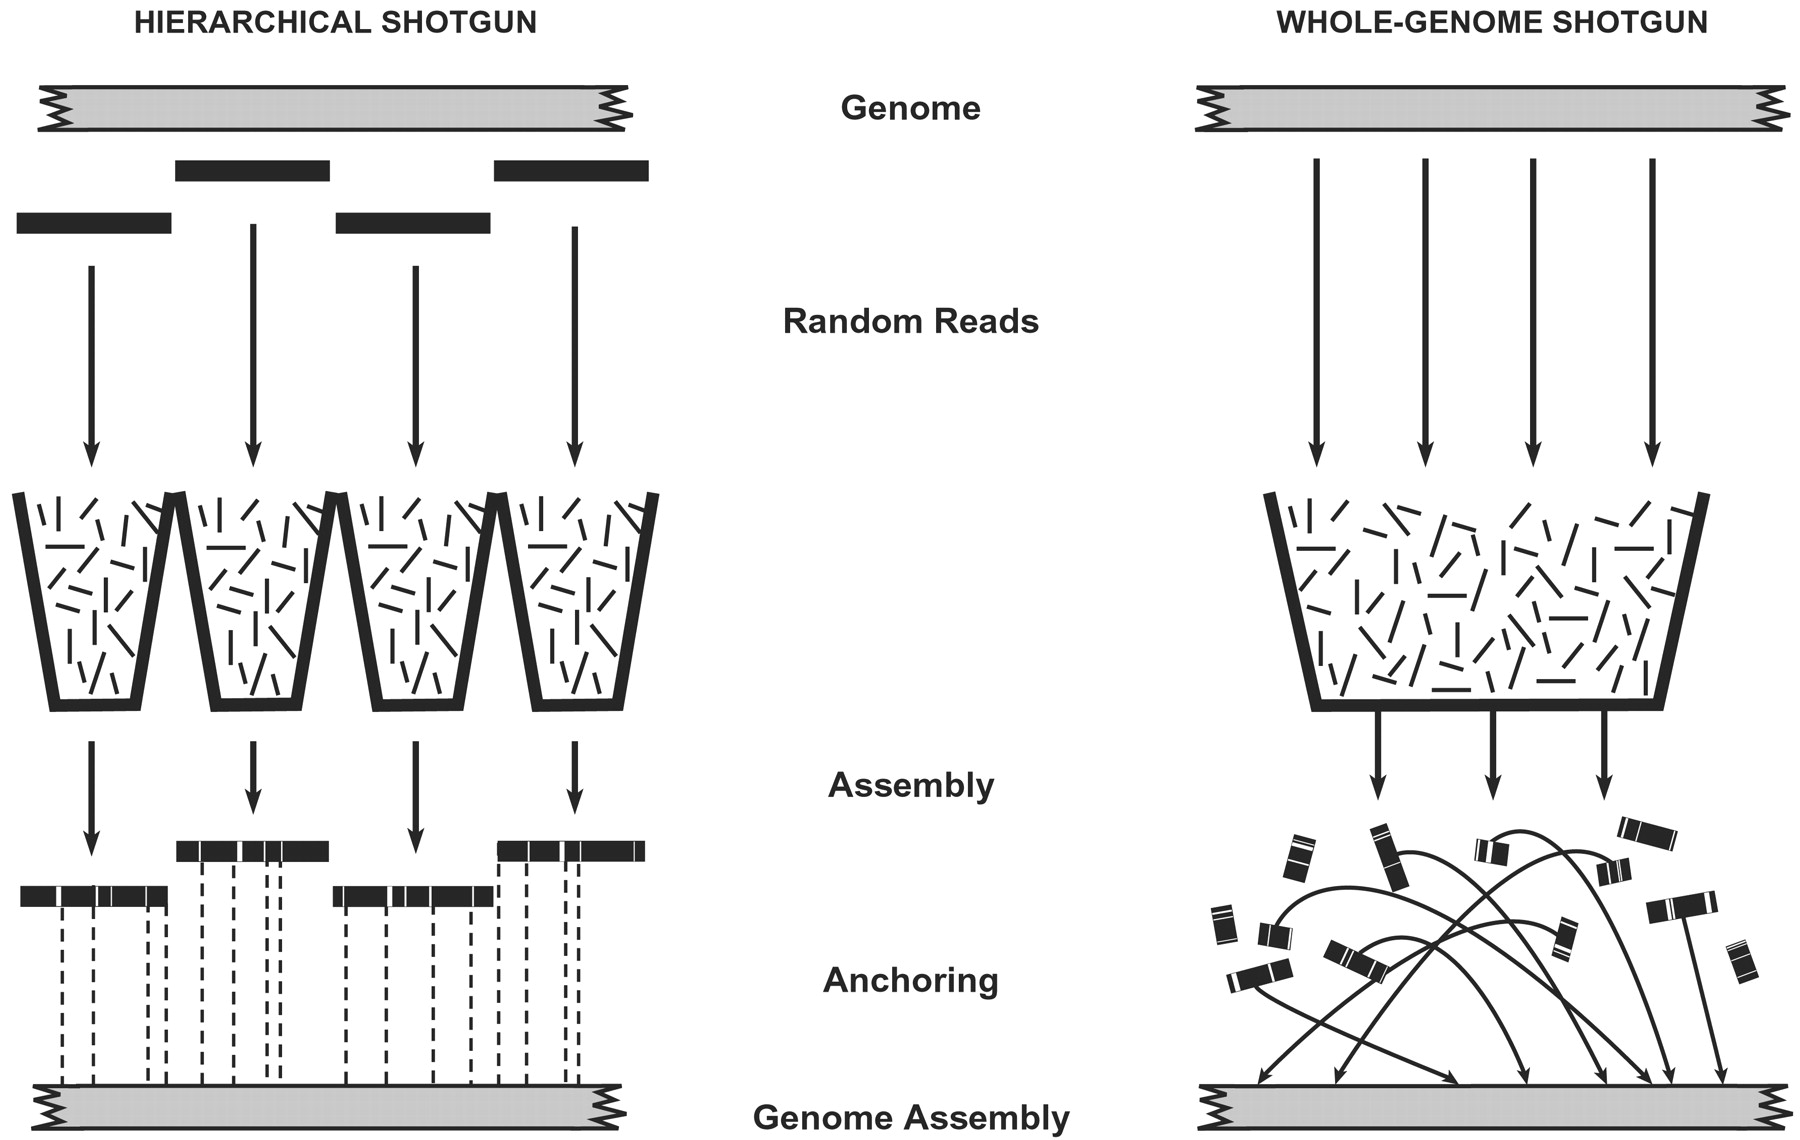
\includegraphics[width=0.9\textwidth]{img/shotguns}
\end{center}
}

\frame
{
\frametitle{Hierarchical Shotgun Sequencing}
\begin{center}
	\huge{Video}
\end{center}
}

\section{Comparación de las técnicas}
%La ventaja para el enfoque jerárquico es que los secuenciadores tienen 
%menos probabilidades de cometer errores al ensamblar los fragmentos 
%``shotgun'' contiguos, mientras sean cromosomas completos. La razón es 
%que la localización cromosómica de cada BAC es conocido, y hay menos
% piezas montadas al azar. La desventaja de este método es tiempo y 
%dinero. El método de la ``shotgun'' es más rápido y menos costoso, pero 
%es más propenso a errores debido a la construcción o montaje de la 
%secuencia final. Por ejemplo, si una porción de 500 kb de un cromosoma 
%se duplica y cada duplicación se corta en fragmentos de 2 KB, entonces
% sería difícil determinar cuando un particular, de 2 piezas kb debe 
%estar ubicado en la secuencia terminada, ya que ocurre dos veces. Se
% podría pensar, "a quién le importa ya que son duplicados? Pero rara 
%vez duplicaciones mantenienen sus secuencias originales, sino que tienden
% a la deriva con el tiempo. Así que una pequeña región se podrá mantener,
% mientras que otras partes pueden mutar. Esto puede crear secuencias de 
%superposición de piezas pequeñas que se encuentran varios cientos de kb 
%de distancia en el cromosoma.
%
%¿Qué método es mejor? Depende del tamaño y la complejidad del genoma.
% Con el genoma humano. Sólo tenemos secuencias de proyecto y cada uno tiene lagunas y 
%regiones sin terminar por lo que no es posible decir con seguridad. 
%Vale la pena mencionar que Celera ha tenido acceso a los datos PGH, pero
% el PGH no tuvo acceso a los datos de Celera. Por otra parte, ya que 
%los datos de Celera no es de libre disposición, la mayoría de los 
%investigadores utilizarán la secuencia de HGP para futuras investigaciones.
% Por lo tanto, nunca puede saber qué método "ganado".


\frame
{
\begin{center}
	\Huge{Comparación}
\end{center}
}

\frame
{
\frametitle{Hierarchical Shotgun vs Shotgun}
\framesubtitle{Principales diferencias}
\begin{center}
	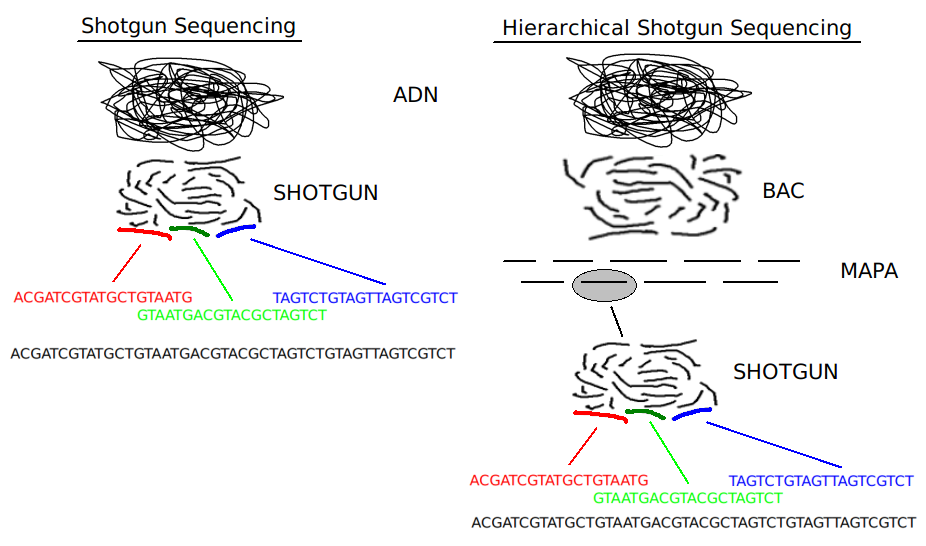
\includegraphics[width=0.9\textwidth]{img/comparacion}
\end{center}
}

\frame
{
\frametitle{Hierarchical Shotgun vs Shotgun}
\framesubtitle{¿Cuál es mejor?}
\begin{itemize}
	\item Depende del tamaño del genoma
	\item Depende de la complejidad del genoma
	\item Depende si se desea exactitud o velocidad.
\end{itemize}
}

\section{Conclusiones}
\frame
{
\frametitle{Conclusiones}

\begin{itemize}
	\item Experiencia muy enriquecedora
	
	\item Baja Autoestima
	
	\item Debido al pequeño tamaño, buen ambiente laboral, con los respectivos conflictos, llevados por indiferencia.
	
	\item Dos perfiles de trabajadores:
	
	\begin{itemize}
		\item aquellos que sólo acatan todo lo que se les dice, 
		\item aquellos que están muy pendiente de si son pasados a llevar en sus derechos
	\end{itemize}

\end{itemize}

}

\frame
{
\frametitle{Conclusiones}

\begin{itemize}

	\item Ciertas figuras, aparte del Jefe, que son de vital importancia para algunas
	personas.
	 
	\item Pese a todos los problemas, puede llegar a convertirse en un equipo con un poco de esfuerzo de cada uno y nuevas medidas realizadas por el jefe para
aumentar el bienestar de sus trabajadores.

\end{itemize}

}

\frame
{
\vspace{2cm}
\begin{center}
	\Huge ¿Preguntas?
\end{center}
}

\end{document}
